\chapter{Desarrollo del modelo y dataset para la navegación mediante segmentación semántica}\label{ch:desarrollo-del-modelo-y-dataset-para-la-navegacion-mediante-segmentacion-semantica}

Como ya ha sido tratado en los capítulos anteriores de este documento, el modelo propuesto de navegación mediante segmentación semántica estará basado en el modelo propuesto por \texttt{PirlNav}\citep{ramrakhya2023} con las modificaciones indicadas en la figura



\begin{equation}
  floor(\frac{255*255*255}{num\_categories})\label{eq:constant}
\end{equation}
\begin{figure}
    \centering
    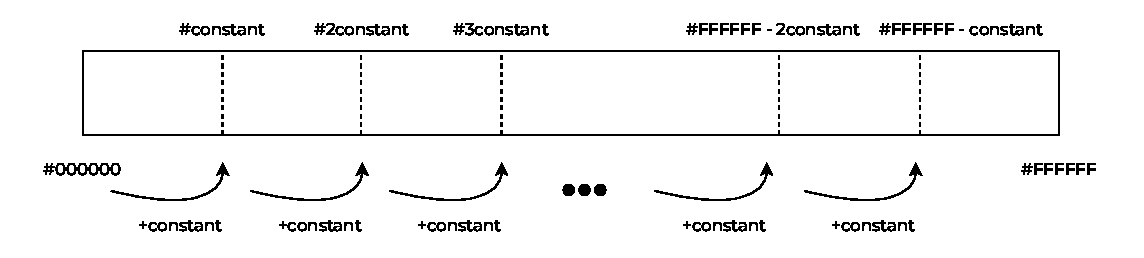
\includegraphics[width=\textwidth]{figuras/colored_scheme.drawio}
    \caption{Esquema de generación de colores mediante la suma de la constante producida por la ecuación\ref{eq:constant}.}
    \label{fig:constant_scheme}
\end{figure}
\begin{figure}
    \centering
    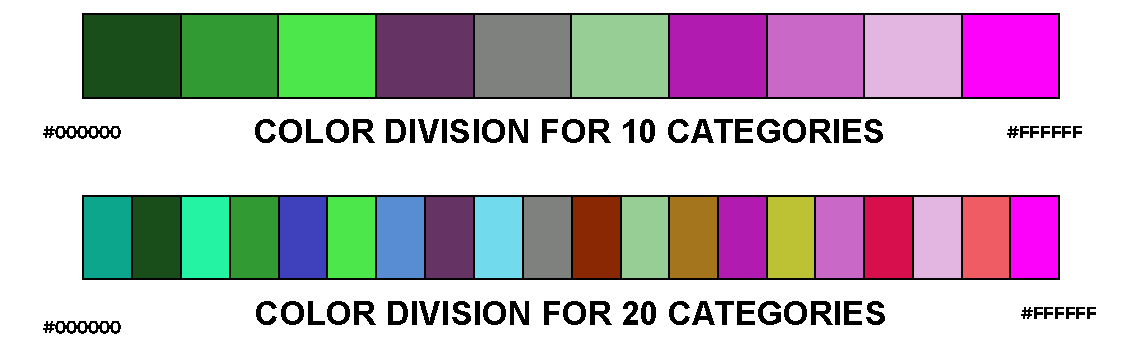
\includegraphics[width=\textwidth]{figuras/morecolored_scheme.drawio}
    \caption{ Ejemplo de generación de colores mediante la estrategia de suma de constante para 10 y 20 categorías.}
    \label{fig:colored_scheme}
\end{figure}
\begin{figure}
    \centering
    \includegraphics[width=0.4\textwidth]{images/vertical_color_gradient_640x480}
    \caption{ Fotografía generada mediante estrategia de división del espectro del color.}
    \label{fig:colorinchis}
\end{figure}